\documentclass{article}
\usepackage{tikz,amsmath,siunitx}
\usepackage{pgfplots}
\usepackage{listings}
\usetikzlibrary{arrows,snakes,backgrounds,patterns,matrix,shapes,fit,calc,shadows,plotmarks}
\topmargin -1.5cm        % read Lamport p.163
\oddsidemargin -0.04cm   % read Lamport p.163
\evensidemargin -0.04cm  % same as oddsidemargin but for left-hand pages
\textwidth 16.59cm
\textheight 21.94cm 
%\usepackage[graphics,tightpage,active]{preview}
%\PreviewEnvironment{tikzpicture}
%\PreviewEnvironment{equation}
%\PreviewEnvironment{equation*}
\title{CS540 Assignment 3}
\author{Dustin Ingram}
\newlength{\imagewidth}
\newlength{\imagescale}
\pagestyle{empty}
\thispagestyle{empty}
\lstset{breaklines=true}
\begin{document}
\maketitle
\newpage
\section{Introduction}
For this assignment, various methods of mini- matrix multiplication optimization are compared, including SSE2 vectorization and multithreading using OpenMP. The results are compared based on the performance.
\section{Summary of Results}
The results can be organized as follows:
\subsection{SSE2 vs. OpenMP vs. Original}
It was found that threadnig the vectorized matrix multiplication offered the highest performance levels. 
\section{Description of Computing Platform}
All tests were run on \texttt{float.cs.drexel.edu}. Relevant system architecture information follows.
\subsection{System \& Kernel Information}
\begin{lstlisting}
$ uname -a
Linux float.cs.drexel.edu 2.6.35-28-generic #50-Ubuntu SMP Fri Mar 18 18:42:20 UTC 2011 x86_64 GNU/Linux
\end{lstlisting}
\subsection{GCC Version Information}
\begin{lstlisting}
$ gcc --version
gcc (Ubuntu/Linaro 4.4.4-14ubuntu5) 4.4.5
\end{lstlisting}
\subsection{CPU Information}
\begin{lstlisting}
$ cat /proc/cpuinfo
processor	: 15
vendor_id	: GenuineIntel
cpu family	: 6
model		: 44
model name	: Intel(R) Xeon(R) CPU           L5630  @ 2.13GHz
stepping	: 2
cpu MHz		: 1600.000
cache size	: 12288 KB
physical id	: 1
siblings	: 8
core id		: 10
cpu cores	: 4
apicid		: 53
initial apicid	: 53
fpu		: yes
fpu_exception	: yes
cpuid level	: 11
wp		: yes
flags		: fpu vme de pse tsc msr pae mce cx8 apic sep mtrr pge mca cmov pat pse36 clflush dts acpi mmx fxsr sse sse2 ss ht tm pbe syscall nx pdpe1gb rdtscp lm constant_tsc arch_perfmon pebs bts rep_good xtopology nonstop_tsc aperfmperf pni pclmulqdq dtes64 monitor ds_cpl vmx smx est tm2 ssse3 cx16 xtpr pdcm dca sse4_1 sse4_2 popcnt aes lahf_lm ida arat dts tpr_shadow vnmi flexpriority ept vpid
bogomips	: 4266.84
clflush size	: 64
cache_alignment	: 64
address sizes	: 40 bits physical, 48 bits virtual
power management:
\end{lstlisting}
\subsection{Memory Information}
\begin{lstlisting}
$ papi_mem_info
Memory Cache and TLB Hierarchy Information.
------------------------------------------------------------------------
TLB Information.
  There may be multiple descriptors for each level of TLB
  if multiple page sizes are supported.

L1 Instruction TLB:
  Page Size:           2048 KB
  Number of Entries:      7
  Associativity:       Full

L1 Instruction TLB:
  Page Size:           4096 KB
  Number of Entries:      7
  Associativity:       Full

L1 Data TLB:
  Page Size:              4 KB
  Number of Entries:     64
  Associativity:          4

L1 Data TLB:
  Page Size:           2048 KB
  Number of Entries:     32
  Associativity:          4

L1 Data TLB:
  Page Size:           4096 KB
  Number of Entries:     32
  Associativity:          4

L1 Instruction TLB:
  Page Size:              4 KB
  Number of Entries:     64
  Associativity:          4


Cache Information.

L1 Data Cache:
  Total size:            32 KB
  Line size:             64 B
  Number of Lines:      512
  Associativity:          8

L1 Instruction Cache:
  Total size:            32 KB
  Line size:             64 B
  Number of Lines:      512
  Associativity:          4

L2 Unified Cache:
  Total size:           256 KB
  Line size:             64 B
  Number of Lines:     4096
  Associativity:          8

L3 Unified Cache:
  Total size:         12288 KB
  Line size:             64 B
  Number of Lines:   196608
  Associativity:         16

mem_info.c                               PASSED
\end{lstlisting}

\newpage
\section{Experiments Performed \& Results}
\subsection{SSE2 vs. OpenMP vs. Original}
This is relatively self-explanatory. Matrix-multiplication was implemented using just SSE2, and then parallelized using OpenMP. The results are as follows, comparing them with the original triply-nested loop (I also included the best blocked-matrix multiply results for additional comparison).\\

\pgfplotsset{width=15cm,compat=1.4}
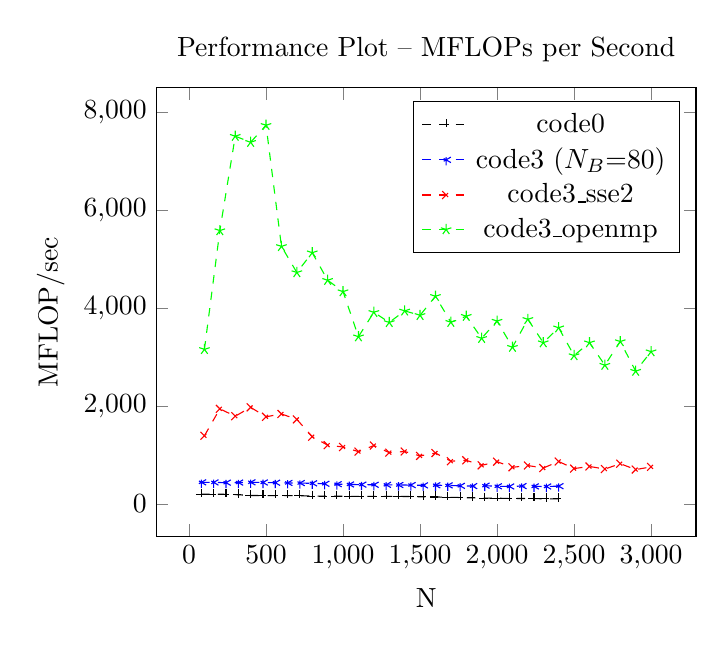
\begin{tikzpicture}
\begin{axis}[
xlabel=N,
ylabel=MFLOP/sec,
legend pos=north east,
title=Performance Plot -- MFLOPs per Second] 
\legend{code0, code3 ($N_{B}$=80), code3\_sse2, code3\_openmp}

\addplot[color=black,mark=+,dashed] coordinates {
(	80	,	197.6929826255	)
(	160	,	198.8440728155	)
(	240	,	196.8224896797	)
(	320	,	188.1825815155	)
(	400	,	173.5493932539	)
(	480	,	170.3740100077	)
(	560	,	169.7130381458	)
(	640	,	169.8101313916	)
(	720	,	169.2183857305	)
(	800	,	160.4442840376	)
(	880	,	158.5767076941	)
(	960	,	157.1294912172	)
(	1040	,	156.300815689	)
(	1120	,	155.6551119783	)
(	1200	,	153.8961007297	)
(	1280	,	154.1316348082	)
(	1360	,	154.6040968069	)
(	1440	,	150.9996898904	)
(	1520	,	146.3545865429	)
(	1600	,	143.0928800391	)
(	1680	,	136.8428730177	)
(	1760	,	132.0082614054	)
(	1840	,	124.4330371376	)
(	1920	,	117.8187102184	)
(	2000	,	117.2567412855	)
(	2080	,	111.9249619669	)
(	2160	,	111.7427307871	)
(	2240	,	109.0673289854	)
(	2320	,	105.3859142508	)
(	2400	,	104.2266883241	)
};


\addplot[color=blue,mark=asterisk,dashed] coordinates {
(	80	,	441.7612256255	)
(	160	,	440.1008662297	)
(	240	,	435.3765785147	)
(	320	,	437.5152088763	)
(	400	,	442.2635087243	)
(	480	,	438.6197551725	)
(	560	,	434.111853641	)
(	640	,	429.652173514	)
(	720	,	427.0278890761	)
(	800	,	421.558623503	)
(	880	,	412.5919956455	)
(	960	,	404.5267891833	)
(	1040	,	398.093315741	)
(	1120	,	395.0690858718	)
(	1200	,	392.3096683068	)
(	1280	,	390.5074520388	)
(	1360	,	387.2639163414	)
(	1440	,	385.7928507693	)
(	1520	,	379.7288574217	)
(	1600	,	382.281538138	)
(	1680	,	379.8389658498	)
(	1760	,	370.3545090199	)
(	1840	,	364.9944786306	)
(	1920	,	373.681025872	)
(	2000	,	361.0888843925	)
(	2080	,	357.4152401079	)
(	2160	,	365.211591731	)
(	2240	,	358.8383452208	)
(	2320	,	356.8971823979	)
(	2400	,	363.6938715545	)
};

\addplot[color=red,mark=x,dashed] coordinates {
(	100	,	1393.94	)
(	200	,	1944.3694785388	)
(	300	,	1793.8700216466	)
(	400	,	1974.9547900435	)
(	500	,	1782.2134554149	)
(	600	,	1839.9195946193	)
(	700	,	1728.7471669291	)
(	800	,	1374.9130086238	)
(	900	,	1201.8990434156	)
(	1000	,	1164.3673906124	)
(	1100	,	1069.9002379135	)
(	1200	,	1193.8530126953	)
(	1300	,	1048.9853217785	)
(	1400	,	1072.1981920838	)
(	1500	,	981.4875426111	)
(	1600	,	1041.194093561	)
(	1700	,	873.7049893849	)
(	1800	,	892.6944208011	)
(	1900	,	789.0495413781	)
(	2000	,	864.2576781425	)
(	2100	,	749.0476066141	)
(	2200	,	785.6739276596	)
(	2300	,	734.4108495716	)
(	2400	,	867.6202571033	)
(	2500	,	723.2408046295	)
(	2600	,	766.669232086	)
(	2700	,	713.2054323811	)
(	2800	,	823.1242497629	)
(	2900	,	702.638740172	)
(	3000	,	757.7355181624	)
};

\addplot[color=green,mark=star,dashed] coordinates {
(	100	,	3160.7191703601	)
(	200	,	5589.222965967	)
(	300	,	7518.8609307076	)
(	400	,	7395.7078865719	)
(	500	,	7742.6255048332	)
(	600	,	5265.9266530247	)
(	700	,	4731.9348613821	)
(	800	,	5137.1150025697	)
(	900	,	4574.200164196	)
(	1000	,	4341.4807681103	)
(	1100	,	3419.5206131271	)
(	1200	,	3918.6174407111	)
(	1300	,	3711.6876096516	)
(	1400	,	3947.4980132759	)
(	1500	,	3856.5640936727	)
(	1600	,	4246.3220178713	)
(	1700	,	3716.0453129928	)
(	1800	,	3838.4644515365	)
(	1900	,	3387.5780556141	)
(	2000	,	3739.4570521415	)
(	2100	,	3205.5976236867	)
(	2200	,	3775.1352182203	)
(	2300	,	3298.5562382122	)
(	2400	,	3602.6106436099	)
(	2500	,	3034.3468247358	)
(	2600	,	3297.0510036618	)
(	2700	,	2838.2513334226	)
(	2800	,	3320.4811873755	)
(	2900	,	2715.4945213013	)
(	3000	,	3114.0769102857	)
};

\end{axis}
\end{tikzpicture}

This reveals, as expected, that vectorization with SSE2 greatly improves speed, and that matrix multiplication is embarrassingly parallelizable when used with a library such as OpenMP for multi-threading.  

\subsection{Source Code \& Data}
An explanation of the source used to generate these graphs as well as the resulting data is contained in the included tarball in the \texttt{README} file.

\section{Conclusion}
To conclude, a number of observations can be made: 
\begin{itemize}
    \item Vectorization and multithreading both greatly improve performance.
\end{itemize}
\end{document}

